\chapter{Introduçao}

Desde os primeiros registros datados, civilizações já observavam o céu e, desse modo, podiam contabilizar a passagem do tempo, identificar as estações do ano, os ciclos sazonais de chuvas e/ou secas, etc. Assim, por exemplo, era possível realizar um planejamento mais assertivo acerca da melhor época de plantio e colheita de diferentes culturas. Cada civilização tinha seu meio e técnica de observação. Por exemplo, em 4000 a.C., os povos da Mesopotâmia utilizavam zigurates para observar o céu noturno; já em 2500 a.C., foi construída a estrutura de pedras Stonehenge, na Inglaterra, para registrar os solstícios. Foi somente em 1609 d.C. que Galileu conseguiu aperfeiçoar e utilizar um telescópio refrator para observar os planetas e as estrelas pela primeira vez \cite{site:brescolaAstrofoto}.

A astrofotografia consiste no emprego de técnicas fotográficas para registrar objetos astronômicos, como planetas, estrelas, galáxias, nebulosas, etc. A primeira astrofotografia é datada de 1840 e é um registro da Lua \cite{site:introCabau}. Desse período em diante, a fotografia teve um papel muito importante na observação celeste e no registro do céu para análise científica. Essa técnica foi evoluindo gradualmente de forma que, por volta de 1960, já havia equipamentos que permitiam realizar registros mais concretos e eficientes, possibilitando fotos com mais definição e nitidez \cite{site:importanciaAstroftoSantos}.

No fim do século XX, telescópios maiores e mais complexos, instalados na Terra ou a orbitando no espaço (como o telescópio espacial Hubble), ampliaram a capacidade da ciência em estudar fenômenos astronômicos ou mesmo a origem do próprio universo \cite{site:importanciaAstroftoSantos}.
Paralelamente, as ferramentas amadoras para astronomia (como telescópios de baixo custo), ou mesmo para astrofotografia (câmeras de custo mais acessível e equipamentos para rastreamento do céu) continuaram a ser desenvolvidas, de forma que um grande número de astrônomos e, especificamente, astrofotógrafos amadores continuassem exercendo seu \textit{hobby} ou mesmo contribuindo à ciência.

Nesse sentido, o desenvolvimento de equipamentos acessíveis voltados ao público amador tem um papel fundamental para despertar o interesse pela ciência em cada vez mais pessoas. Atualmente, o custo de muitas ferramentas classificadas como “amadoras” ainda é elevado, principalmente para a realidade brasileira. Como exemplo, hoje podem ser empregados pequenos telescópios comerciais ou artesanais acoplados a câmeras digitais (de celular ou DSLRs-(Digital Single Lens Reflex). No entanto, os principais desafios de se fotografar galáxias, nebulosas, etc., é que esses corpos, de forma geral, demandam elevados tempos de exposição \cite{site:introCabau}. Infelizmente, o movimento de rotação da Terra não permite que os astros sejam expostos ao sensor por muito tempo, pois as imagens ficariam borradas. Por esse motivo, é necessário o uso de uma ferramenta que movimente a câmera (acoplada ou não a um telescópio) no sentido de rotação aparente do céu, compensando o movimento e permitindo que o sensor da câmera possa receber luz por longos períodos de tempo (de minutos a horas) \cite{site:introCabau}. Assim, consegue-se obter um registro fotográfico de alta qualidade e com um baixo custo computacional de pós processamento.


Por isso, existem inúmeras ferramentas comerciais para o rastramento do céu voltadas ao público amadador, como Nyx Track, SkyGuiderTM Pro, PolarieTM, entre outras (conforme Figura \ref{fig:skyguider}). Porém, todas elas são comercializadas no hemisfério norte e com um custo excessivo para brasileiro médio (considerando taxa de câmbio, taxas de importação e frete). Assim, de modo a contribuir à popularização da astrofotografia no Brasil, incentivando cada vez mais jovens a seguirem na carreira científica, propõe-se o desenvolvimento de uma plataforma equatorial de baixo custo para astrofotografia.


\begin{figure}[htb]
	\centering
	\caption{Exemplo de solução comercial empregada em astrofotografias. }
	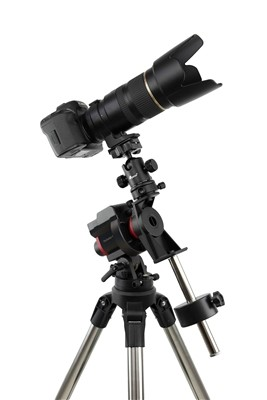
\includegraphics[width=0.3\linewidth]{figuras/skyguider}
	\label{fig:skyguider}
	\fonte{\cite{site:ioptron}}
\end{figure}
